\documentclass[10pt,twocolumn,letterpaper]{article}

\usepackage{cvpr}
\usepackage{times}
\usepackage{epsfig}
\usepackage{graphicx}
\usepackage{subfigure}
\usepackage{listings}
\usepackage{algorithm}
\usepackage{algorithmic}
\usepackage{multirow}
\usepackage{amsmath}
\usepackage{rotating}
\usepackage[margin=0.75in]{geometry}
\usepackage{amssymb}

% Include other packages here, before hyperref.

% If you comment hyperref and then uncomment it, you should delete
% egpaper.aux before re-running latex.  (Or just hit 'q' on the first latex
% run, let it finish, and you should be clear).
\usepackage[pagebackref=true,breaklinks=true,letterpaper=true,colorlinks,bookmarks=false]{hyperref}


%\cvprfinalcopy % *** Uncomment this line for the final submission

\def\cvprPaperID{1516} % *** Enter the CVPR Paper ID here
\def\httilde{\mbox{\tt\raisebox{-.5ex}{\symbol{126}}}}

% Pages are numbered in submission mode, and unnumbered in camera-ready
\ifcvprfinal\pagestyle{empty}\fi
\begin{document}


%%%%%%%%
%% Title
%%%%%%%%
\title{Object Localization Enhancement by Multiple Segmentations Fusion}

\author{Ahmed Mounir Gad, Ramon Baldrich\\
Universitat Autonoma de Barcelona,\\
Barcelona, 08193, Spain\\
{\tt\small \{amounir,ramon\}@cvc.uab.es}
}

\maketitle
% \thispagestyle{empty}

%%%%%%%%%%%
%% Abstract
%%%%%%%%%%%
\begin{abstract}

Despite being a complex task, image segmentation is a crucial prerequisite for many computer vision applications,
including object tracking, object recognition and object localization.
Image segmentation is known to be unstable because it is highly affected by image perturbations such as shadows, shading and highlights.
In our work, we effeciently combine different cues from multiple segmentations of an image to obtain a better segmentation and, hence, better localization.
We propose a novel framework for object class segmentation that
(i) combines different complementary cues from multiple segmentations in a bottom-up fashion
and
(ii) augments the power of the bottom-up segmentation by fusing multiple segmentations in a top-down approach.
To combine multiple segmentations in a bottom up fashion we propose an efficient evaluation criteria for assessing the quality of the generated segments.
We refer to it ``segments goodness measure''.
On the other hand, for fusing multiple segmentations in a top-down fashion we introduce a novel ``voting'' technique  that assigns each segment to its corresponding category.
Finally, we discuss some possible extensions for our method that could potentially boost the performance.
Our results exceed state-of-the-art results on PASCAL VOC 2007 object segmentation dataset.

\end{abstract}

\section{Introduction}

Image segmentation is a computer vision process focusing on
partitioning an image into a set of non-overlapping regions. This is
an extremely challenging task for real images. The shape variations of
the objects provoke several effects related with the illumination such
as shadows, shadings and highlights. These effects are one of the main
problems that should be solved in order to obtain an efficient
segmentation.

Image segmentation algorithms can be divided in several ways, however,
all of the existing approaches can first be divided into two main
hierarchies: bottom-up approaches and top-down approaches.

Bottom-up segmentation approaches mainly examine the image and try to
figure out how to divide it into coherent and meaningful segments.
Comprehensive surveys as presented in \cite{Yz_colorimage,Cheng01colorimage}
drew the basis for the current classification of bottom-up segmentation
techniques. From all of these existing methods, segmentation methods can
be divided into four main categories: feature-based, image-based,
physics based and hybrid approaches.

Feature based approaches mainly focus on the photometric information of
an image represented by its histogram as in the work by
\cite{1059188,Yang07unsupervisedsegmentation}. Image-based approaches
exploit the spatial coherence of color in an image. An example is given
from the work of \cite{649319}. Physics-based methods use physics and
psychophysics information to perform the segmentation. Finally, hybrid
techniques combine methods of the previous categories.

Top-down approaches, on the other hand, are guided primarily by high-level
information and the use of class-specific criteria. The motivation for
using these class-specific criteria, as shown by \cite{649285}, has two
parts. The first is that although recent image segmentation algorithms
provide impressive results, they still often fail to capture meaningful
and at times crucial parts of the objects in the image. The second is that
these methods are analogous to human vision in the sense of indicating
high-level, class-based criteria to segment the images in a meaningful
manner. Examples of using top-down approaches to perform segmentation are
shown in the work of \cite{649285,Leibe04combinedobject,1097721}.

Image segmentation has been applied to solve a variety of computer vision problems.
A robust and efficient segmentation is an important preprocessing step for several
computer vision tasks. However, extensive experiments by \cite{Unnikrishnan_2007_5789}
show that when using a single region generated by an image segmentation
algorithm, the segmentation quality is highly variant and dependent on image
data, the segmentation algorithms and the parameters used to create this
segmentation. This was a motivation for the emerging new trend in object
recognition that uses the segments generated from multiple segmentation
algorithms and tries to merge them efficiently to recognize objects in the
scene \cite{Efros_2006_5395,PSH08,malisiewicz-bmvc07}.

This trend of using multiple segmentations was also the motivation for our work.
In our work we focus on two parts. The first one is building a robust and
efficient segmentation method. This method uses the information provided by
several other segmentation algorithms to build a more reliable image segmentation
in a bottom-up fashion. The second is using this new segmentation along with the
other segmentation methods to recognize and localize objects in the image. We
perform object class segmentation using each segmentation method separately.
Afterwards, we combine the results in a top-down approach.

The goal of object class image segmentation is to produce a pixel-level
classification of the input image. In other words, it is required to indicate
which class does each pixel lie into. In figure \ref{fig:obj_seg} we show
an example of object class image segmentation. This is a highly constrained
problem where most state-of-the-art approaches focus on exploiting contextual
information available around each pixel. Afterwards, they measure feature
statistics from this information (in this case histograms of visual words)
and use the bag-of-words technique in order to determine the class that
each pixel belongs to.

\begin{figure}
\centering
\subfigure[] {
    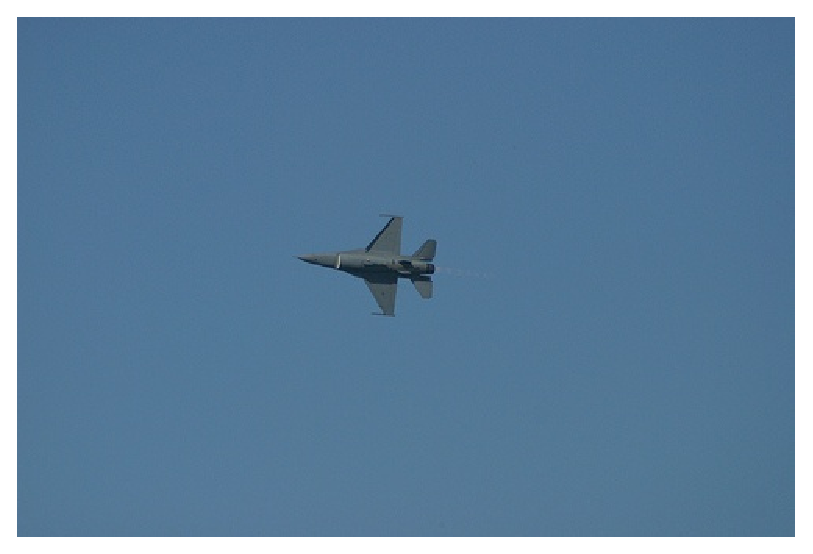
\includegraphics[width=50pt,height=40pt]{./Figures/forg1.eps}
    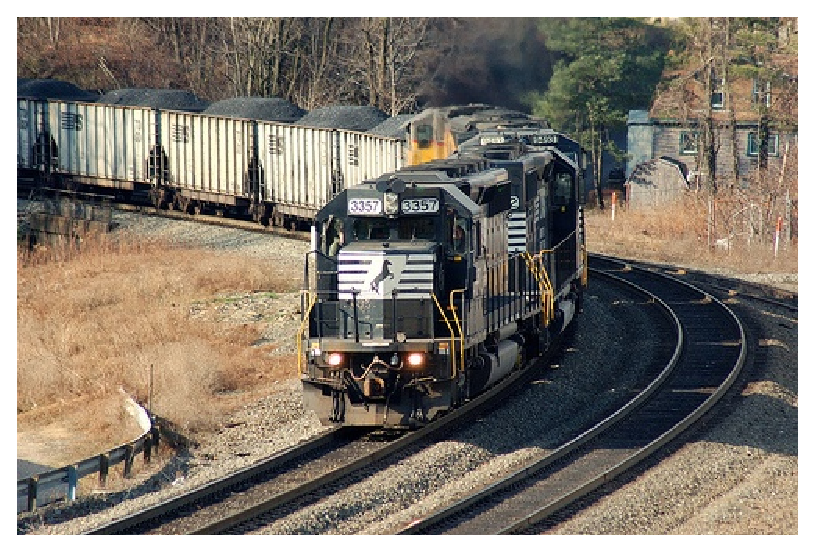
\includegraphics[width=50pt,height=40pt]{./Figures/forg2.eps}
    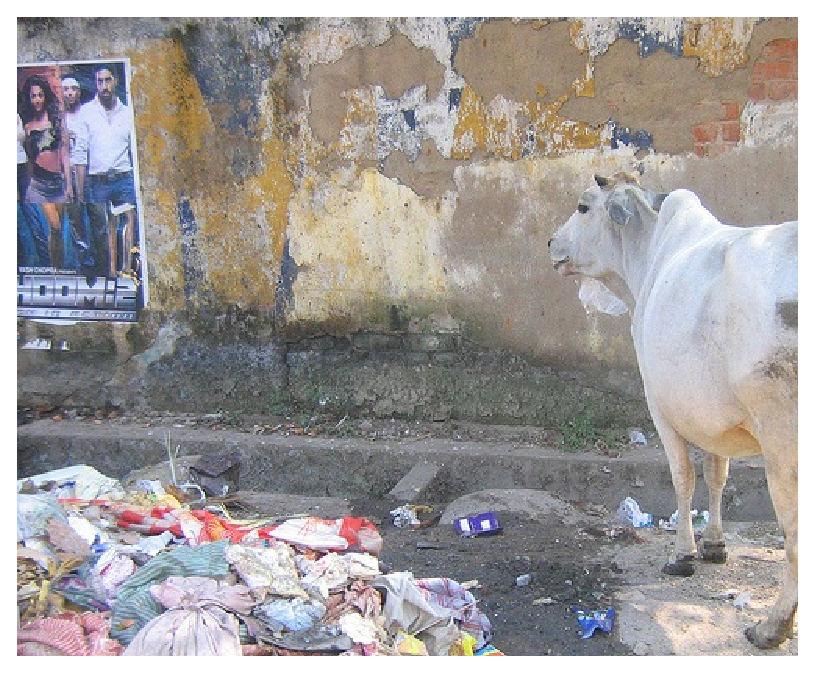
\includegraphics[width=50pt,height=40pt]{./Figures/forg3.eps}
    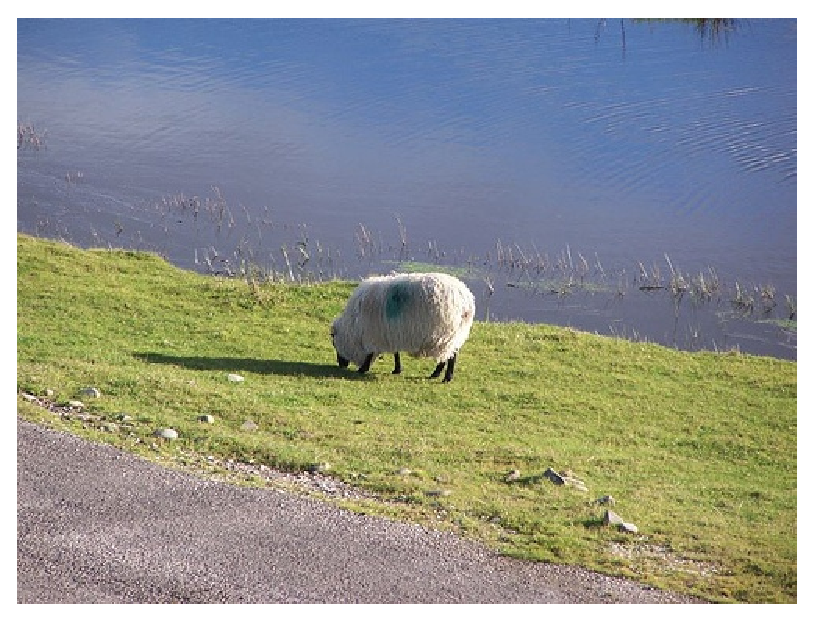
\includegraphics[width=50pt,height=40pt]{./Figures/forg4.eps}
    \label{fig:classsegorg}
}\\
\subfigure[] {
    
\includegraphics[width=50pt,height=40pt]{./Figures/gt1.eps}
    
\includegraphics[width=50pt,height=40pt]{./Figures/gt2.eps}
    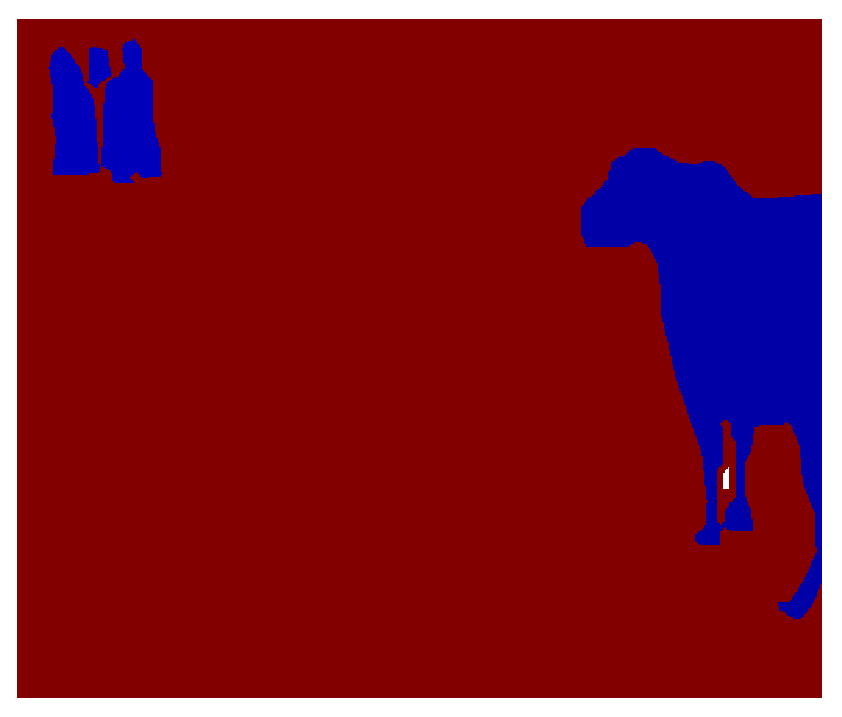
\includegraphics[width=50pt,height=40pt]{./Figures/gt3.eps}
    
\includegraphics[width=50pt,height=40pt]{./Figures/gt4.eps}
    \label{fig:classseggt}
}
\caption{(a) Original images (b) Object class segmentation}
\label{fig:obj_seg}
\end{figure}

Instead of working on pixels, Fulkerson et al. in \cite{fulkerson09class}
present a method to perform object class segmentation by aggregating the
histograms in the neighborhood of the small regions obtained from a conservative
over-segmentation, or ``superpixels'' \cite{Ren03learninga,4587471}.
They don't use the information obtained by superpixels alone. They also
use information from neighboring superpixels to provide more contextual
information. However, in our work we show that even when adding neighborhood
information, superpixels are still not the best choice for describing an object.

In our work, instead of using pixels or superpixels, we use regions emerging
from several segmentation techniques. Our results show that superpixels do
not capture enough information about the objects being recognized and
localized that can be better captured by using larger segments.
We learn a model from each segmentation method to classify the regions of
this segmentation method. Afterwards, we combine all of the results coming
from each model separately into a new model using our proposed technique that we call,
the ``voting technique''. Our results show that combining results from outputs of
several segmentations that use complementary information give a significant
improvement over using each segmentation method solely. The results are even better
than those obtained using superpixels with aggregating neighborhood information for
classification. Figure \ref{fig:our_obj_seg_model} shows our proposed framework for
approaching the object class segmentation problem.

\begin{figure}[!t]
\centering
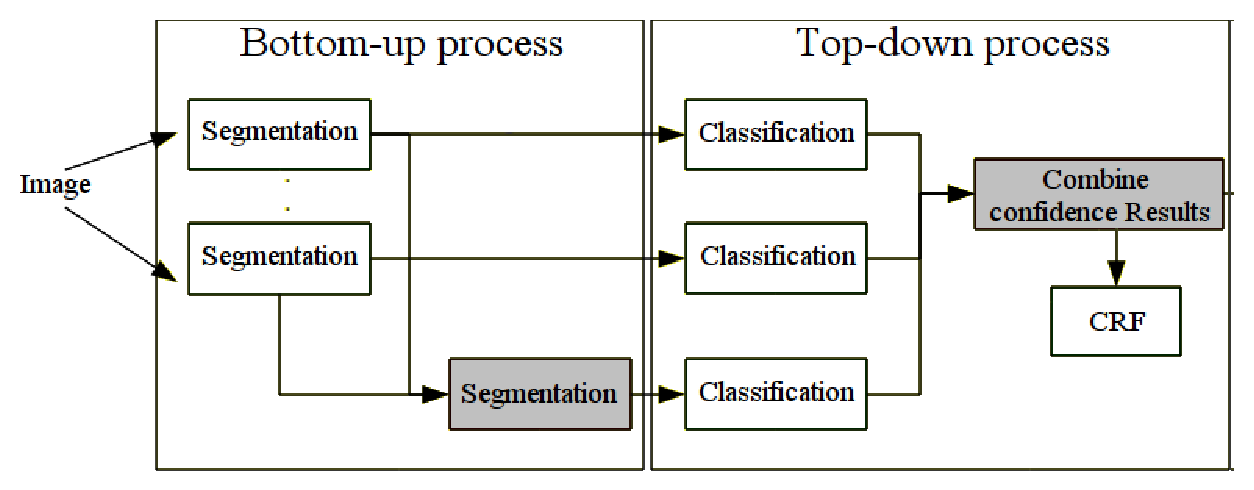
\includegraphics[scale=.4]{./Figures/our_framework.eps}
\caption{Our object class segmentation model. Our contributions are highlighted in grey.}
\label{fig:our_obj_seg_model}
\end{figure}

This paper is organized as follows. In section \ref{GeneratMSeg}, we describe our different
generated segmentation techniques. In section \ref{BuildSeg}, we explain how we combine
different segmentation techniques in a bottom-up fashion to obtain a new segmentation technique.
In section \ref{TopDownComb}, we show how we augment the performance of the bottom-up segmentation
by combining information from multiple segmentations in a top-down fashion.
Our framework relies on VLBlocks \cite{fulkerson09class} framework. We briefly show the
steps for extracting our descriptors in section \ref{ClassifySegs} and for refining our final results
with Conditional Random Field (CRF) in section \ref{sectionCRF}. In section \ref{sectionExperiments},
we'll show our experiments and results. Finally, we'll give our conclusions and future work in
section \ref{sectionConclusions}

\section{Generating Multiple Segmentations}\label{GeneratMSeg}

Our proposed framework makes use of the complementary cues provided by different
segmentation approaches, in order to build a more reliable segmentation. We
generate a segmentation based on mean-shift \cite{Comaniciu02meanshift}.
In this segmentation we guarantee that the segments mainly vary in the color
distribution. In addition, we use the graph-based method
\cite{Felzenszwalb04efficientgraph-based} to guarantee a variation along the edges.
Finally, we benefit from the existence of large segments by using the
normalized cut technique \cite{Shi_2000_3808}.

Using these different and complementary segmentations, we maintain the desired
qualities from each aspect yielding a more robust segmentation model.

To this end, our goal is to: (i) combine these segmentations in a bottom-up
fashion in order to obtain a new more reliable segmentation. (ii) Fuse
these complementary segmentations along with our newly proposed ones in a
top-down fashion for a better final object class segmentation.

\section{Building a More Reliable Segmentation (Bottom-up Fusion)}\label{BuildSeg}

In this section we propose a novel approach for combining multiple segmentations in a bottom-up fashion.
We introduce a segments evaluation method. We refer to it as  ``segment goodness evaluation''.
This method allows us to effectively combine the different segments that emerge from each of the considered segmentation approaches .

Our technique is inspired by the work of Fulkerson et al. \cite{fulkerson09class}.
Instead of applying the neighborhood operator on superpixels, we applied it on segments.
We get these segments from the several segmentation techniques that we previously described (Section \ref{GeneratMSeg}).
We investigated the effect of increasing the neighborhood size for the concerned segmentation techniques on the final average accuracy (Figure \ref{fig:neigh_effect}).

Figure \ref{fig:neigh_effect} illustrates two important conclusions. First, large segments
produce good results. This conclusion is based on the observation of increasing the overall average accuracy in case of
(i) the large segments generated by the normalized cut technique, and
(ii) the generated segments using the superpixels or mean-shift methods when taking larger neighborhood size into account.

The second conclusion is that up to a certain limit, increasing the size of the segments or the neighborhood, decrease the final average accuracy.
We attribute this to the loss of semantic information due to the combination of segments that are no longer related to each others.
Consequently, our target is to find a criteria to decide whether combining smaller segments or splitting larger ones is more useful.

\begin{figure}
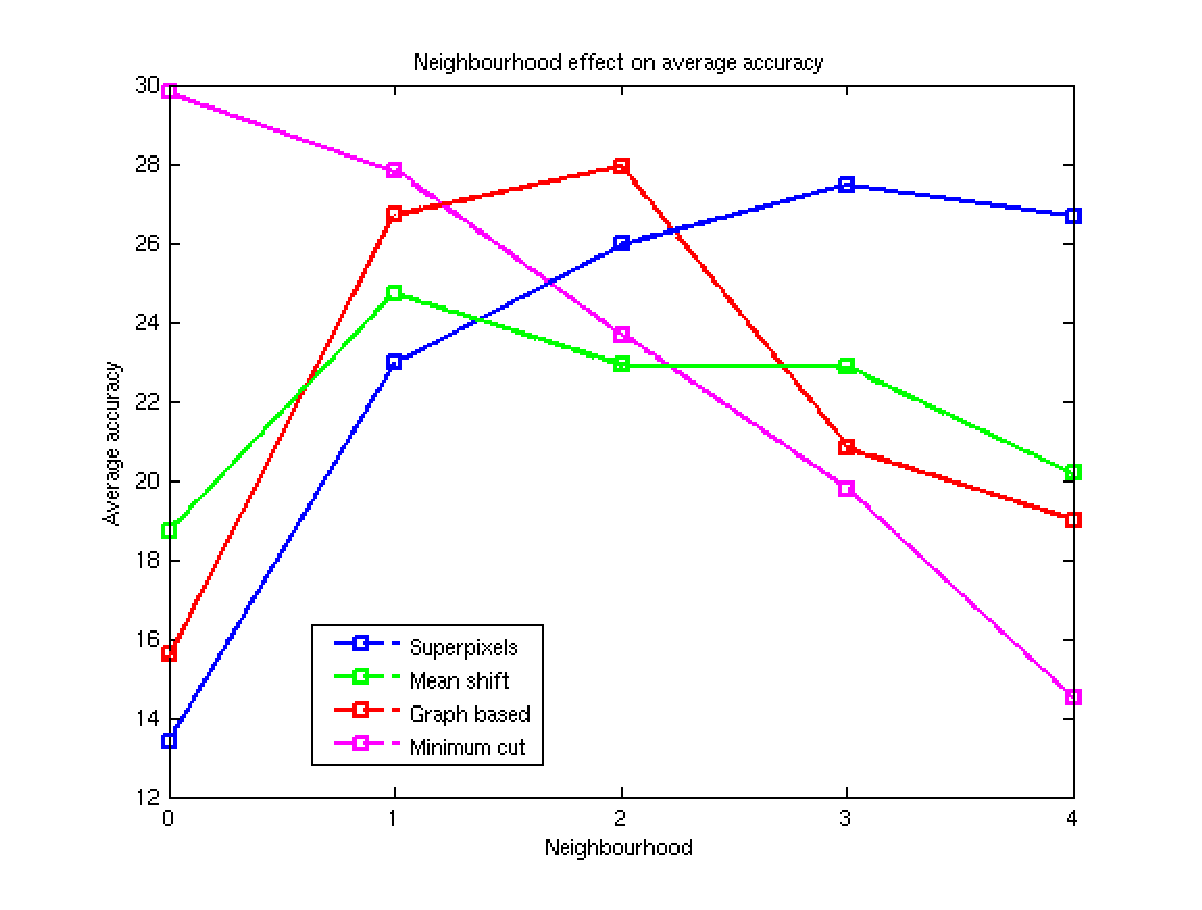
\includegraphics[width=200pt,height=160pt]{./Figures/neigh_acc.eps}
\centering
\caption{Effect of increasing the neighborhood on the average accuracies}
\label{fig:neigh_effect}
\end{figure}

Assume we have $N$ segmentations $S_i$, where $i = 1, ..., N$ and each of the
segmentations correspond to $S_i = \bigcup_{j=1}^{M_i}T_{ij}$, where $T_ij$ is a
segment in the segmentation $S_i$ and $M_i$ is the number of segments obtained
from the segmentation $S_i$. Our objective is to obtain a better segmentation
$S^* = \bigcup_{k=1}^{M^*}T_k^*$, where $T^*_k$ is a segment in our final set of
optimized segments and $M^*$ is the total number of optimized segments. Segmentation
$S^*$ should satisfy the following criteria:

\begin{enumerate}
\item
The segments of the final segmentation should be as large as possible. In other
words, we need to minimize $M^*$.
\item
The segments should be ``good'' segments. In our context, we defined a ``good
segment'' as the largest set of connected pixels that lie in the same class.
\end{enumerate}

Consequently, our motivation for combining segmentations is to start looking for
the large segments and then check if this segment is a ``good'' segment. We
applied a greedy algorithm that favors large segments and check if they pass a
certain criteria of ``goodness''.
Our proposed approach is described as follows:
We examine the largest segment obtained from all segmentations methods and check whether this segment is a ``good'' segment.
If the segment is ``good'', we include it in our final segmentation (Add to $S^*$).
Otherwise, we try to segment it recursively using the least number of segments from the other segmentations.
Similarly, we segment the remaining part of the image.

To this end, we need to determine whether the generated segments are ``good'' or not.
To do this, we investigate several ``goodness'' evaluation criteria.
First, we studied the possibility of assuming that the color of each region should follow a normal distribution.
However, this ``goodness'' criteria didn't hold on real images as shown in figure \ref{fig:histn}.
Second, we examined the unimodality test to check whether the distribution of the histogram of each RGB channel follow a unimodal function.
We use Dip test \cite{dip-unimodality} for unimodality. Although the resulting segments were slightly better than those obtained using the normality test,
it also fails to handle real images' segments as in figure \ref{fig:histn}.
In addition, we also investigated the outliers detection and the Ridge based Distribution Analysis (RAD) methods.
We'll describe each of these three techniques in more details in the next sections.

\begin{figure}[!t]
\centering
\subfigure[] {
    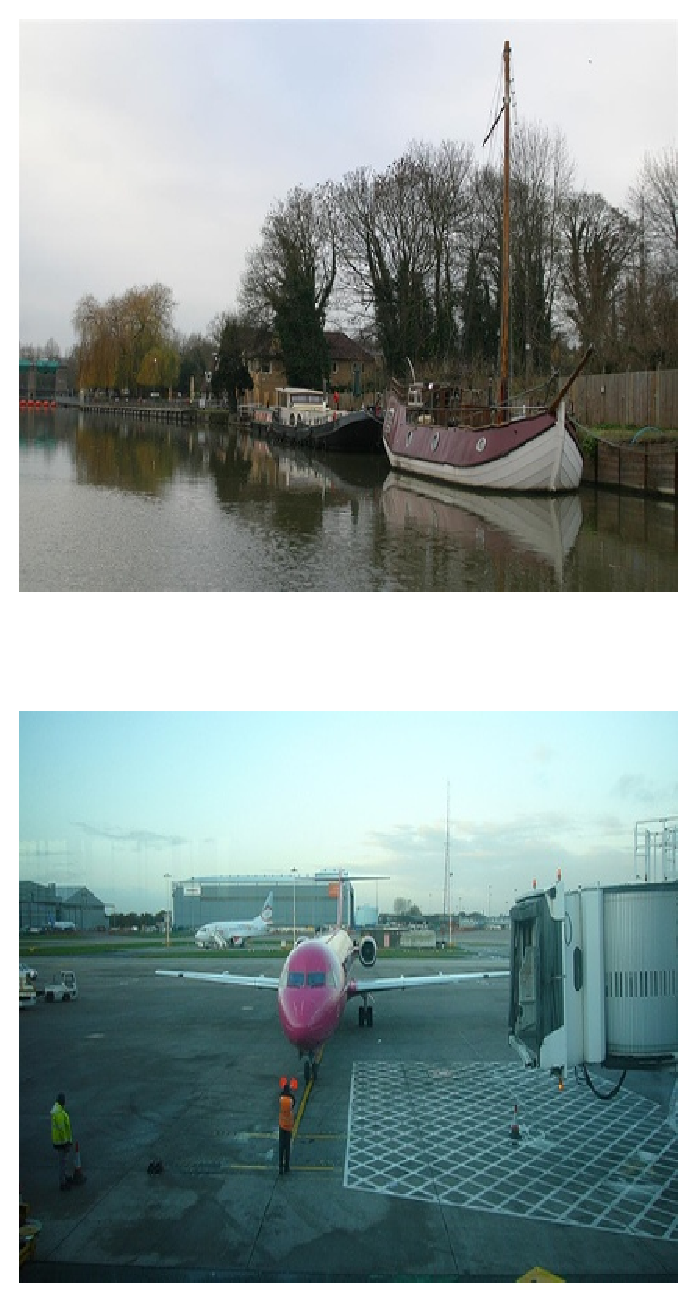
\includegraphics[width=70pt,height=85pt]{./Figures/orgnormality2.eps}
    \label{fig:orgn}
}
\subfigure[] {
    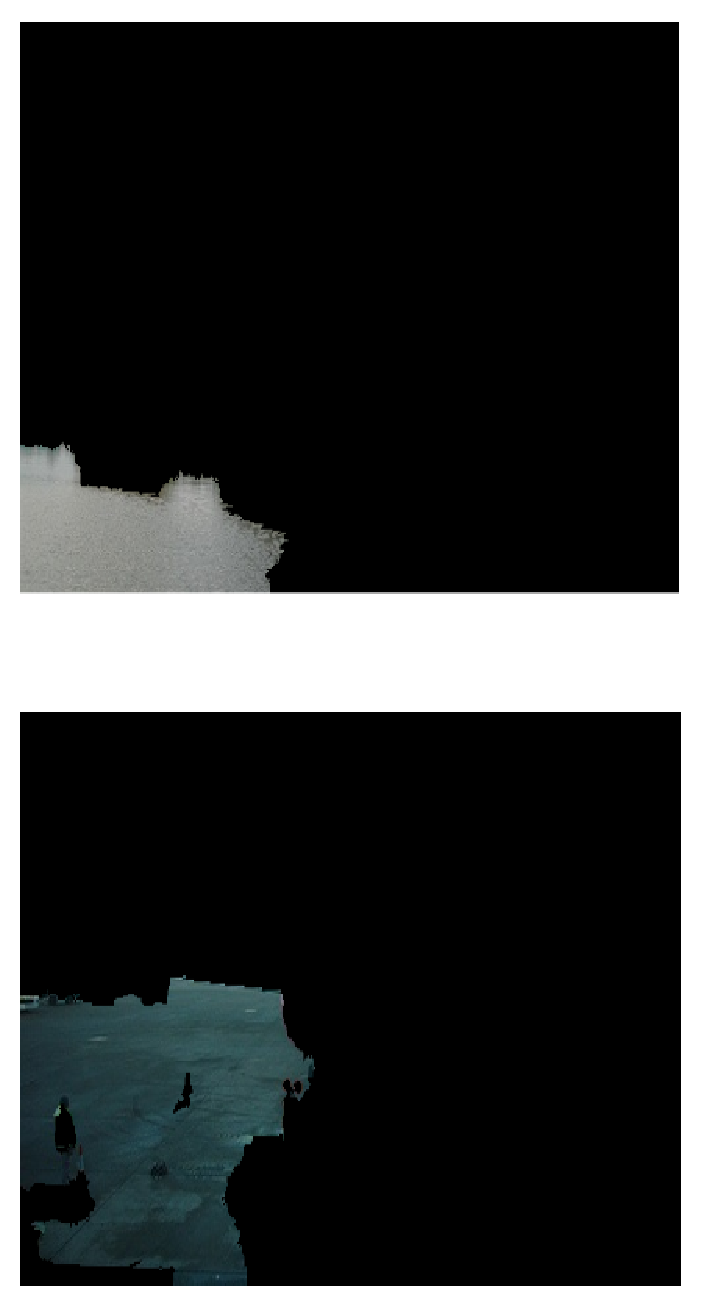
\includegraphics[width=70pt,height=85pt]{./Figures/segnormality2.eps}
    \label{fig:segn}
}
\subfigure[] {
    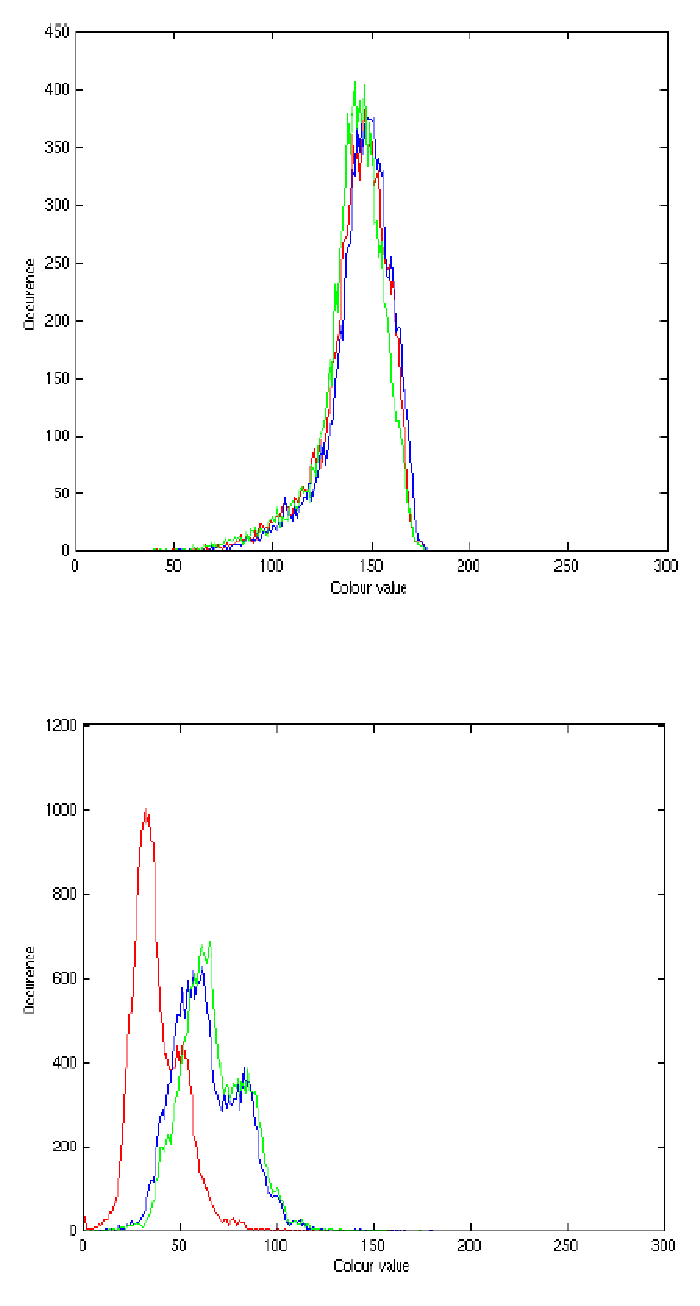
\includegraphics[width=70pt,height=85pt]{./Figures/histnormality2.eps}
    \label{fig:histn}
}
\caption{(a) Original images (b) Current largest segments (c) Histograms from
every channel. As we can see the first image can be approximated into a
normal distribution or a unimodal distribution while the second one fails in
that test.}
\label{fig:colorhists}
\end{figure}

\subsection{Good Segments Evaluation Using Outliers Finding}

As defined by \cite{grubbs-1969}, ``An outlying observation, or outlier, is one
that appears to deviate markedly from other members of the sample in which it
occurs.'' In our work, we consider a segment to be ``good'' if the number of outliers inside this
segment is below a certain threshold. We use the Z-Test to find the outliers of a certain segment. The Z-Test
indicates that the point is considered an outlier if it satisfies the following
formula:

\begin{equation}
\frac{|X - \mu|}{\sigma} > 3,
\end{equation}

where X is a label for each point of a segment in the image, $\mu$ is the mean of the color
values of the considered segment and $\sigma$ is the standard deviation of these colors.

We performed a series of experiments to empirically determine the best value
for the tolerance of outliers inside the segment. We finally decided that a
segment is considered ``good'' if the number of outliers lying inside is less
than $2\%$ of the number of pixels in the segment.

Although outliers detection worked well in detecting the segments shown in Figure
\ref{fig:segn}, they didn't work on detecting the segments that contain variations
in shadows and highlights. Consequently, we examined other evaluation methods
that work well in the presence of shadows and illuminations. For this purpose, we use the
RAD evaluation method due to its robustness to shadows and highlights.

\subsection{Good Segments Evaluation Using RAD}

We use the RAD method presented in \cite{1478239} for obtaining image
segmentations in the presence of shadows and highlights. This method is based on
the insight that the distributions formed by a single-colored object have a
physically determined shape (i.e. follow the same ridge) in the color histogram space \cite{Sha85}.
To capture these ridges Vazquez et al. \cite{1478239} proposed a new Ridge based
Distribution Analysis (RAD) to find the set of ridges representative of the dominant color.

We model the region ``segment'' by its set of dominant colors (DC). This DC is described
by a distribution in histogram-space. We assume that if this segment contains only 1 DC
then this segment is a ``good'' segment as this segment contains only 1 semantic object.
Based on this technique, the evaluation method becomes very robust to shadows and highlights
and becomes closely related to the physical features of each segment than the previously
investigated methods.

To perform this evaluation we use the first step proposed by \cite{1478239} which extracts ridges as a representative
of a dominant structure (DS). Afterwards, we check whether we have only one single
ridge in the considered segment. Accordingly, we consider this segment as a ``good'' segment.

\subsection{Segmentations Evaluation on the Berkeley Dataset and Benchmark}

In this section, we perform a series of experiments on the standard Berkeley Segmentation Dataset and
Benchmark \cite{MartinFTM01}. We evaluate the performance of the three considered segmentation methods with our
newly proposed segmentation method. Our method combines the complementary information obtained by all the
considered segmentation methods using the RAD criteria for segments ``goodness'' evaluation.

We evaluate four different error measurements for evaluating the quality of the segments
generated by our approach. These four error measures are: First, the Probabilistic Rand Index
(PRI) \cite{Unnikrishnan_2007_5789}, which counts the fraction of pairs of pixels whose labellings are
consistent between the computed segmentation and the ground truth, averaging across
multiple ground truth segmentations to account for scale variation in human perception.
The second error measure is the Variation of Information (VoI) \cite{citeulike:3906686}.
It defines the distance between two segmentations as the average conditional entropy
of one segmentation given the other, and thus roughly measures the amount of randomness
in one segmentation which cannot be explained by the other. The third is the Global
Consistency Error (GCE) \cite{MartinFTM01} that measures the extent to which one
segmentation can be viewed as a refinement of the other. Segmentations which are related
in this manner are considered to be consistent, since they could represent the same
natural image segmented at different scales. The fourth measure is the Boundary
Displacement Error (BDE) by \cite{649319}. It measures the average displacement error of
boundary pixels between two segmented images. Particularly, it defines the error of one
boundary pixel as the distance between the pixel and the closest pixel in the other
boundary image.

Table \ref{tab:seg_bench} demonstrates that our proposed segmentation method improves both of the PRI and the VoI error measures.
We attribute this to the fact that  PRI and VoI are clearly concerned about comparing segments entirely with the ground truth segments.
This justifies our motivation behind our proposed segmentation method which is based on improving the size and the quality of the segment.
In contrary, GCE and BDE measures don't perform well on our approach.
These measures are mainly concerned about the boundaries of the segments which our approach doesn't take into concern.

\begin{table}
\centering
\begin{tabular}
{|c||c|c|c|c|}
\hline
               & PRI             & VoI             & GCE             & BDE              \\\hline
Mean-Shift     & 0.7424          & 4.5293          & \textbf{0.0842} & \textbf{14.2716} \\\hline
Graph-Based    & 0.7082          & 5.1148          & 0.1150          & 17.2428          \\\hline
Normalized-cut & 0.7079          & 4.1370          & 0.1153          & 14.7337          \\\hline
Mix+RAD        & \textbf{0.7483} & \textbf{3.5364} & 0.1433          & 14.8047          \\\hline
\end{tabular}
\caption{Segmentation benchmarks results for the Berkeley Segmentation Dataset and
Benchmark. 4 error measures were considered for 4 different segmentations.}\label{tab:seg_bench}
\end{table}

\section{Describing and Classifying Regions From Each Segmentation}\label{ClassifySegs}

Relying on the same framework by Fulkerson et al. \cite{fulkerson09class}, a bag of features
classifier is constructed. It operates on the regions defined by
the segments obtained from each segmentation method. SIFT descriptors are extracted
for each pixel in the image at a fixed scale and orientation.

The extracted descriptor are then quantized using a K-means dictionary and aggregated
into one $l^1$ normalized histogram. For training the classifier, the most frequent class label
contained by each segment is assigned to it. Afterwards,  a one-vs-rest support vector  machine
(SVM) with an RBF-$\chi^2$ kernel is trained on the labeled histograms for each of the object
categories.

The $\chi^2$ distance between histograms $h_1$ and $h_2$ is calculated using
the following formula:

\begin{equation}
d^2_{\chi^2}(h_1,h_2) = \sum_{m=1}^M{\frac{(h_1(m) - h_2(m))^2}{h_1(m) + h_2(m)}}.
\end{equation}

From the previous equation it can be concluded that the larger the segment is,
the more discriminative this distance will become. This is because the larger the
segment will be the more the information it will carry from the dictionary and the
more the variance will be in the final value of the distance which will lead
to better classification.

\section{Combining Region Classifications (Top-down fusion)}\label{TopDownComb}

In this section, we first briefly revisit the approach proposed by Pantofaru et al. \cite{PSH08} to combine multiple segmentations.
Firstly, pixels that are grouped together by every segmentation should be classified consistently.
These groups of segmentations are called Intersection of Regions (IofRs).
Secondly, these IofRs are consistently classified based on the information obtained from their original segments emerging from each of the segmentation techniques.

In our approach, we classify each IofR by combining the information from all of the individual segmentations.
Each classifier results in a confidence map which is then combined together with all individual segmentation results (confidence maps) to obtain a final confidence for each IofR.
Instead of averaging all the confidence maps as in \cite{PSH08}, we adapt a voting methodology that assigns different weights to each instance (category) in a confidence map.
In this way, we construct a weighted confidence map per segmentation.
Consequently, these weighted confidence maps are combined to obtain a final confidence map.
It is noteworthy to mention that instead of simple averaging all the confidence maps, in our approach, each confidence map is weighted by rearranging the confidence values per category.


We now introduce some mathematical notations to formulate our approach:
Let $I$ be a given Image,
$k$ be a certain class label in the set of class labels $\cal{C}$,
$S_s$ be a specific segmentation in the set of segmentations $\cal{S}$,
$r$ be a certain IofR,
$CF_{r,s}$ be the confidence map for the IofR $r$ that indicates for each class $k$, the $P(c_r=k|S_s)$, where $c_r$ is the class label of $r$.
For each IofR, our aim is to construct a set of weights $W_{r,s}^k$ that weighs each class $k$ for each IofR $r$ based on its position $O_{r,s}^k$ in the ordered $CF_{r,s}$.
Thus, the index of a class $k$ in $CF_{r,s}$ can be obtained as:
\begin{eqnarray}
O_{r,s}^k = \#\{P(c_r=t|S_s) > P(c_r=k|S_s)\}_{t\neq{k}}
\end{eqnarray}
Where $t$ is a class label in $\cal{C}$. The probabilities are obtained from our confidence map $CF_{r,s}$.
Our weights are then assigned depending on the value of $O_{r,s}^k$:
\begin{eqnarray}
W_{r,s}^k = H(O_{r,s}^k)
\end{eqnarray}
Where $H(O_{r,s}^k)$ is the weighting function that determines the appropriate weight based on the position $O_{r,s}^k$.
Finally, the class label $c_r$ for each $r$ can be intuited from the following formula:
\begin{eqnarray}\label{eq_class_r}
P(c_r=k|I) \propto \sum_{S_s\in\cal{S}}{W_{r,s}^k}
\end{eqnarray}

From eq. \ref{eq_class_r} the final class assigned to $r$, $C_r$ is expressed as:
\begin{eqnarray}
C_r = \arg\max_k  \sum_{S_s\in\cal{S}}{W_{r,s}^k} 
\end{eqnarray}


Note that the confidence for each IofR is altered based on the probability of it belonging to a certain category.
To calculate $H(O_{r,s}^k)$, a fixed set of weights are then assigned depending on the position $O_{r,s}^k$.
In this work, we keep the weights fixed to $H(p)=\frac{1}{p + 1}$, but this can easily be learned on the validation set through cross-validation.
This way, an improved object class segmentation is obtained as depicted in the figure \ref{fig:qualitativebetter}.
A final confidence map is then obtained by averaging all weighted confidence maps.
%Our approach is explained by Algorithm \ref{alg:votation}. 
In figure \ref{fig:votation} we also show a graphical explanation of this procedure.

\begin{figure}
\subfigure[The voting algorithm.] {
    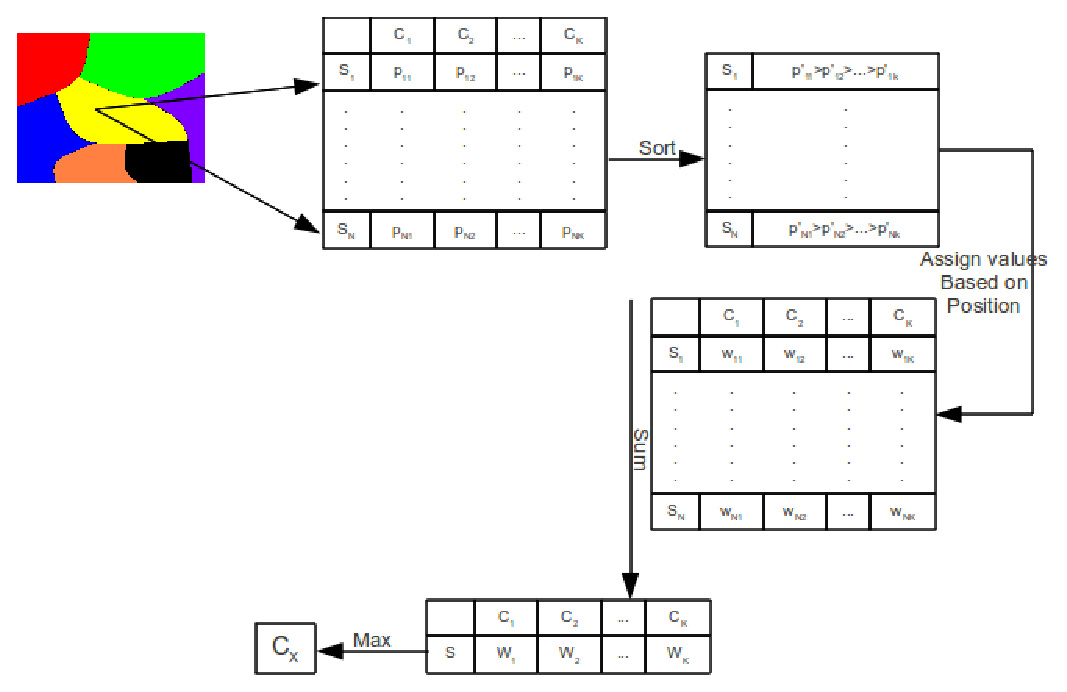
\includegraphics[scale=.45]{./Figures/votation.eps}
}
\subfigure[Combining Mean-Shift, Graph-Based and Normalized-cut segmentations resulted in a better segmentation.] {
    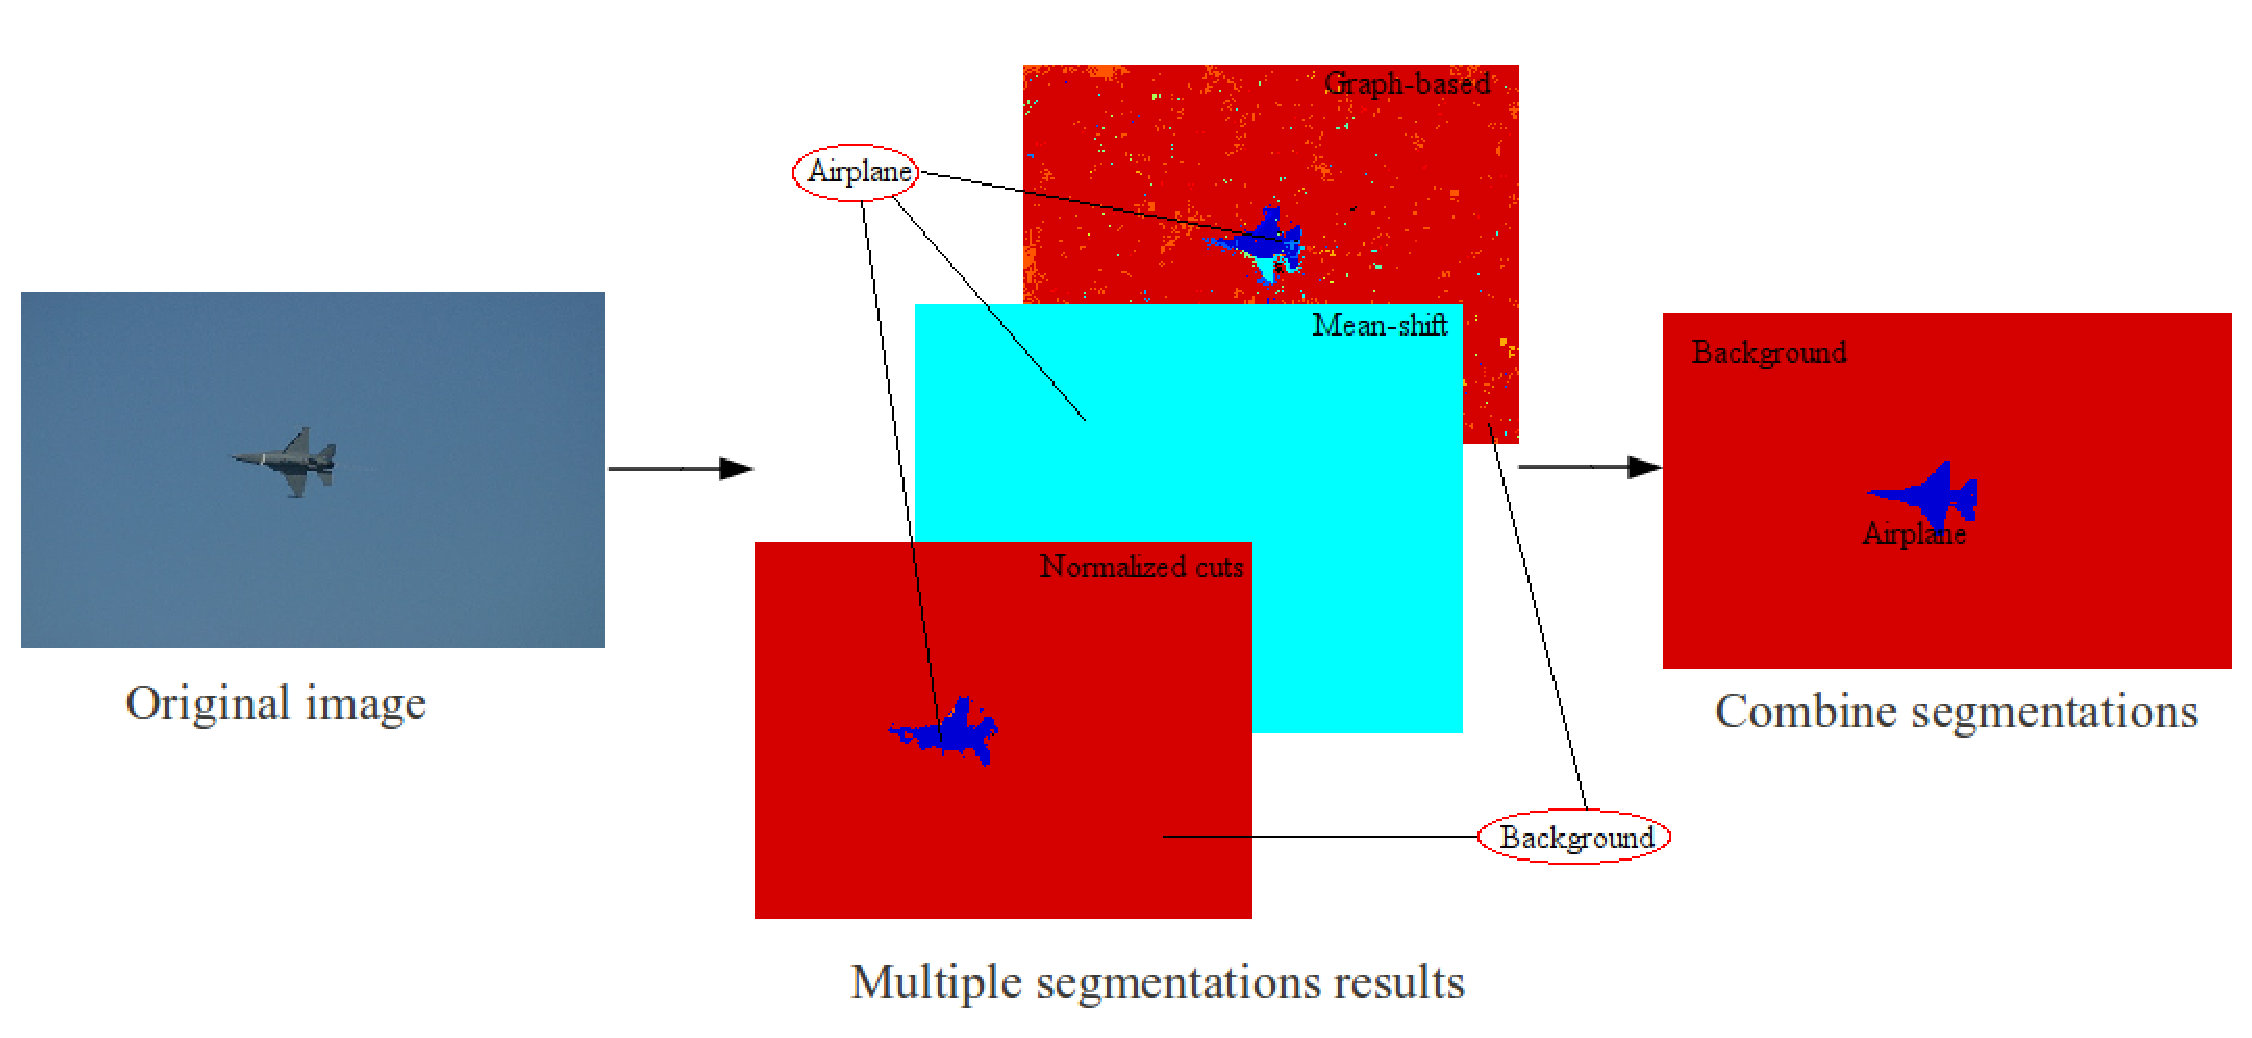
\includegraphics[scale=.22]{./Figures/qualitative.eps}
    \label{fig:qualitativebetter}
}
\centering
\label{fig:votation}
\caption{Voting scheme illustrated}
\end{figure}

%\begin{algorithm}
%\caption{Getting Class Label for IofR}
%\begin{algorithmic}
%\STATE Initialize weights map $W$
%\FORALL {$s$ in $S$}
%\STATE Get $i_r^s$
%\FORALL {$k$ in $K$}
%\STATE $O_k^i = \#\{P(c_i=t|I) > P(c_i=k|I)\}_{t\neq{k}}$
%\STATE $W_i^k = H(O_k^i)$
%\STATE $W[k] = W[k] + W_i^k$
%\ENDFOR
%\ENDFOR
%\RETURN $MAX(W)$
%\end{algorithmic}
%\label{alg:votation}
%\end{algorithm}

\section{Refining Results With a CRF}\label{sectionCRF}

This is the final step of our framework. In order to recover more precise boundaries
and reduce the effects of mis-classifications inside the image, we finally refined
our results with a conditional random field.

In our framework, we used the same technique explained in \cite{fulkerson09class}.
However, instead of working on segments emerging from superpixels, we worked on Intersection of Regions (IofRs) as our basic units.
Our formulas are similar to \cite{fulkerson09class}. They are included again for the sake of clarity.
However, instead of applying the CRF on superpixels, we apply them on IofRs.

Assume the final segmentation $G(I, E)$ where $I$ is an Intersection of Regions
in an adjacency graph. $P(c|G;w)$ is the conditional probability of the set of
class label assignments $c$ where $w$ is a weight.

\begin{eqnarray}
-log(P(c|G;w)) & = & \sum_{I_i\in{S}}{\psi(c_i|I_i)} \nonumber \\
& + & \omega{\sum_{(I_i, I_j)\in{E}}{\phi(c_i,c_j|I_i,I_j)}}.
\end{eqnarray}

The unary potentials $\psi$ are obtained from probability outputs provided
by our SVM for each segment:

\begin{equation}
\psi(c_i,I_i) = -log(P(c_i|I_i)),
\end{equation}

and the pairwise edge potentials $\phi$ are obtained using the following formula:

\begin{equation}
\phi(c_i,c_j|I_i,I_j) = (\frac{L(I_i,I_j)}{1 + \parallel{I_i} - I_j\parallel})[c_i\neq{c_j}],
\end{equation}

where $\parallel{I_i} - I_j\parallel$ is the norm of the color difference
between the two neighboring IofRs in the LUV colorspace. $L(I_i,I_j)$
is the shared boundary length between IofRs $I_i$ and $I_j$ and acts as
a regularizing term discouraging small regions.

\section{Experiments}\label{sectionExperiments}

We evaluated our method on the standard PASCAL VOC 2007 \cite{pascal-voc-2007} segmentation competition data set.
This dataset contains multiple object classes with extreme variation in deformation, scale,
illumination, pose and occlusion. While the challenge specifies that the
detection challenge training data may also be used, we use only the 422 fully
segmented images to train our core approach. The performance measure for this
dataset is the average pixel accuracy: for each category the number of correctly
classified pixels is divided by the ground truth pixels plus the number of
incorrectly classified pixels. We also show the total percentage of pixels
correctly classified.

Our results are divided into three main parts.
In the first one we show the obtained results for combining the considered segmentation techniques
in a bottom up fashion using different evaluation criteria, namely: Outliers and RAD.
Follwing this, we show the effect of combining the considered segmentation results in a top-down fashion.
We don't include our newly created segmentation method that aims to look for larger segments.
Finally, we include our new segmentation method and show its effect on the overall average accuracy.

\begin{table*}
\centering
\begin{tabular}{|@{ }c@{ }||@{ }c@{ }|@{ }c@{ }|@{ }c@{ }|@{ }c@{ }|@{ }c@{ }|@{
}c@{ }|@{ }c@{ }|@{ }c@{ }|@{ }c@{ }|@{ }c@{ }|@{ }c@{ }|@{ }c@{ }|@{ }c@{ }|@{
}c@{ }|@{ }c@{ }|@{ }c@{ }|@{ }c@{ }|@{ }c@{ }|@{ }c@{ }|@{ }c@{ }|@{ }c@{ }||@{
}c@{ }|}\hline
& {\begin{sideways}Background\end{sideways}} &
{\begin{sideways}Airplane\end{sideways}} &
{\begin{sideways}Bicycle\end{sideways}} & {\begin{sideways}Bird\end{sideways}} &
{\begin{sideways}Boat\end{sideways}} & {\begin{sideways}Bottle\end{sideways}} &
{\begin{sideways}Bus\end{sideways}} & {\begin{sideways}Car\end{sideways}} &
{\begin{sideways}Cat\end{sideways}} & {\begin{sideways}Chair\end{sideways}} &
{\begin{sideways}Cow\end{sideways}} &
{\begin{sideways}Dinningtable\end{sideways}} &
{\begin{sideways}Dog\end{sideways}} & {\begin{sideways}Horse\end{sideways}} &
{\begin{sideways}Motorbike\end{sideways}} &
{\begin{sideways}Person\end{sideways}} &
{\begin{sideways}Pottedplant\end{sideways}} &
{\begin{sideways}Sheep\end{sideways}} & {\begin{sideways}Sofa\end{sideways}} &
{\begin{sideways}Train\end{sideways}} &
{\begin{sideways}TVmonitor\end{sideways}} & {\begin{sideways}Avg
Accuracy\end{sideways}}\\\hline
Outliers                & 22 & 9  & 15 & 8  & 25 & 14 & 18 & 11 & 43 & 11 & 13 & 16 & 31 & 22 & 27 & 6  & 31 & 15 & 35 & 27 & 18 & 20\\
RAD                     & 26 & 12 & 11 & 26 & 17 & 16 & 28 & 17 & 53 & 14 & 14 & 40 & 28 & 21 & 50 & 20 & 50 & 38 & 30 & 50 & 32 & 28\\\hline
Voting (MS+NC+GB)       & 48 & 20 & 21 & 16 & 10 & 30 & 32 & 42 & 56 & 23 & 19 & 35 & 51 & 18 & 63 & 52 & 28 & 20 & 29 & 40 & 34 & 33\\
\cite{PSH08} (MS+NC+GB) & 38 & 30 & 21 & 11 & 14 & 9  & 25 & 24 & 61 & 36 & 21 & 14 & 53 & 24 & 65 & 52 & 27 & 15 & 31 & 42 & 42 & 31\\\hline
Voting + RAD            & 49 & 21 & 20 & 10 & 15 & 9  & 32 & 48 & 56 & 28 & 13 & 37 & 56 & 19 & 61 & 48 & 33 & 32 & 45 & 44 & 38 & \textbf{34}\\
\cite{tkk_pascal}       & 23 & 19 & 21 & 5  & 16 & 3  & 1  & 78 & 1  & 3  & 1  & 23 & 69 & 44 & 42 & 0  & 65 & 40 & 35 & 89 & 71 & 30\\
\cite{fulkerson09class} & 56 & 26 & 29 & 19 & 16 & 3  & 42 & 44 & 56 & 23 & 6  & 11 & 62 & 16 & 68 & 46 & 16 & 10 & 21 & 52 & 40 & 32\\
\cite{PSH08}            & 59 & 27 & 1  & 8  & 2  & 1  & 32 & 14 & 14 & 4  & 8  & 32 & 9  & 24 & 15 & 81 & 11 & 26 & 1  & 28 & 17 & 20\\\hline
\end{tabular}
\caption{MS = Mean-Shift, GB = Graph-Based, NC = Normalized-Cut. Comparison on the average accuracy for different
segmentation algorithms, segmentations created using other segmentations, combining already existing segmentations
and combining all segmentations with newly created segmentations.}
\label{tab:allsegs}
\end{table*}

\subsection{Parameters Setup}

In our experiments, we use VLBlocks \cite{fulkerson09class}. Furthermore, we added our
extra modules for combining segmentations in various ways. In this section, we'll explain in more details
the different parameters chosen in our experiments.

\subsubsection{Framework Parameters}

We used the same framework proposed by Fulkerson et al. \cite{fulkerson09class}.
We extract SIFT descriptors at each pixel using the quick SIFT technique in
the VLFeat framework \cite{vedaldi08vlfeat}. The patch size for the SIFT
descriptors is 12 pixels. Descriptors are quantized into a K-means dictionary
learned using the training data. $K = 400$ was chosen for all of the performed
experiments.

For training, labels are assigned to training segments coming from each segmentation by the
majority of class votes that we get from our training ground truth. We randomly
select an equal number of training histograms from each category as the training
data for our SVM. We learn a one-versus-rest SVM model for each class with an RBF-$\chi^2$. We
used the libSVM tool \cite{libsvm}. Finally, we refined our final labeled
results with a CRF model as described in section \ref{sectionCRF}.

\subsubsection{Multiple Segmentations Parameters}

In this section we explain the parameters used for the different segmentations that we
take in concern. We evaluated three types of segmentations,
Mean-shift segmentation \cite{Comaniciu02meanshift}, Graph-based segmentation
\cite{Felzenszwalb04efficientgraph-based} and normalized cut segmentation \cite{Shi_2000_3808}.

For the mean-shift segmentation we use the EDISON wrapper
\cite{Christoudias02synergismin}. This code requires the following parameters:
$hs$, indicating the spatial bandwidth for mean shift analysis,
$hr$, indicating the range bandwidth for mean shift analysis
and $M$ which is the minimum size of final output regions.
For our experiments we use $hs = 11$, $hr = 8$ and $M = 40$.

For the efficient Graph-Based (GB) image segmentation we use the code in
\cite{Felzenszwalb04efficientgraph-based}.
The following parameters are required: $threshold$, the larger this value is, the larger the segmented area becomes.
$minsize$, indicates the minimum size of segmentation component.
$nRadius$, the radius of neighborhood of a pixel.
We use the following values. $threshold = 0.5$, $minsize = 50$, and $nRadius = 2$.

For the minimum cut we use the version explained by the work of \cite{1069213}.
The framework requires the number of requested segments as its parameter.
We chose the value of $100$ to be the number of requested segments each time.

We generate an over-segmentation to obtain superpixels using quickshift \cite{vedaldi08quick}
These superpixels are controlled with the following three parameters:
$\lambda$, the trade-off between color importance and spatial importance,
$\sigma$, the scale at which the density is estimated
and $\tau$ the maximum distance in the feature space between members of the same region.
In our experiments we use the following parameters, $\lambda = 0.5$, $\sigma = 2$ and, $\tau = 8$.

In all our segmentations we chose our values after we applied several tries on the validation set and manually tuned the
parameters in order to find the best description for the segments and their boundaries.

\subsection{Results}

First, we evaluated the different methods proposed for combining segments in a bottom-up fashion.
We clearly show that the RAD criteria for ``segments goodness'' evaluation outperforms the other method
that searches for outliers inside the segments.

Following this, we we evaluated our voting technique by combining the mean-shift, graph-based and normalized-cut
segmentations. We compared it against the method described in \cite{PSH08}. We extracted the same features under
the same conditions and we show that our ``voting technique'' outperforms the results obtained from combining
the segments using the method in \cite{PSH08}.

Finally, we incorporate the voting method with our newly created segmentation method's results and we compare it
with the state-of-the-art results. Our results show a significant improvement over state of the art approaches on a
number of classes. It also shows an improvement for the overall average accuracy.

Table \ref{tab:allsegs} demonstrates our results. It's clearly seen that applying the voting technique by itself
(in the middle portion of the table) outperforms the state of the art results.
Making use of the bottom up segmentation combination into the voting technique yields in boosting the overall performance.

Finally, in figure  \ref{fig:qualitative} we show some qualitative results for our method. We show the original
images along with the confidence for the class it should be assigned to.

\begin{figure}
\subfigure[Ground truth] {
    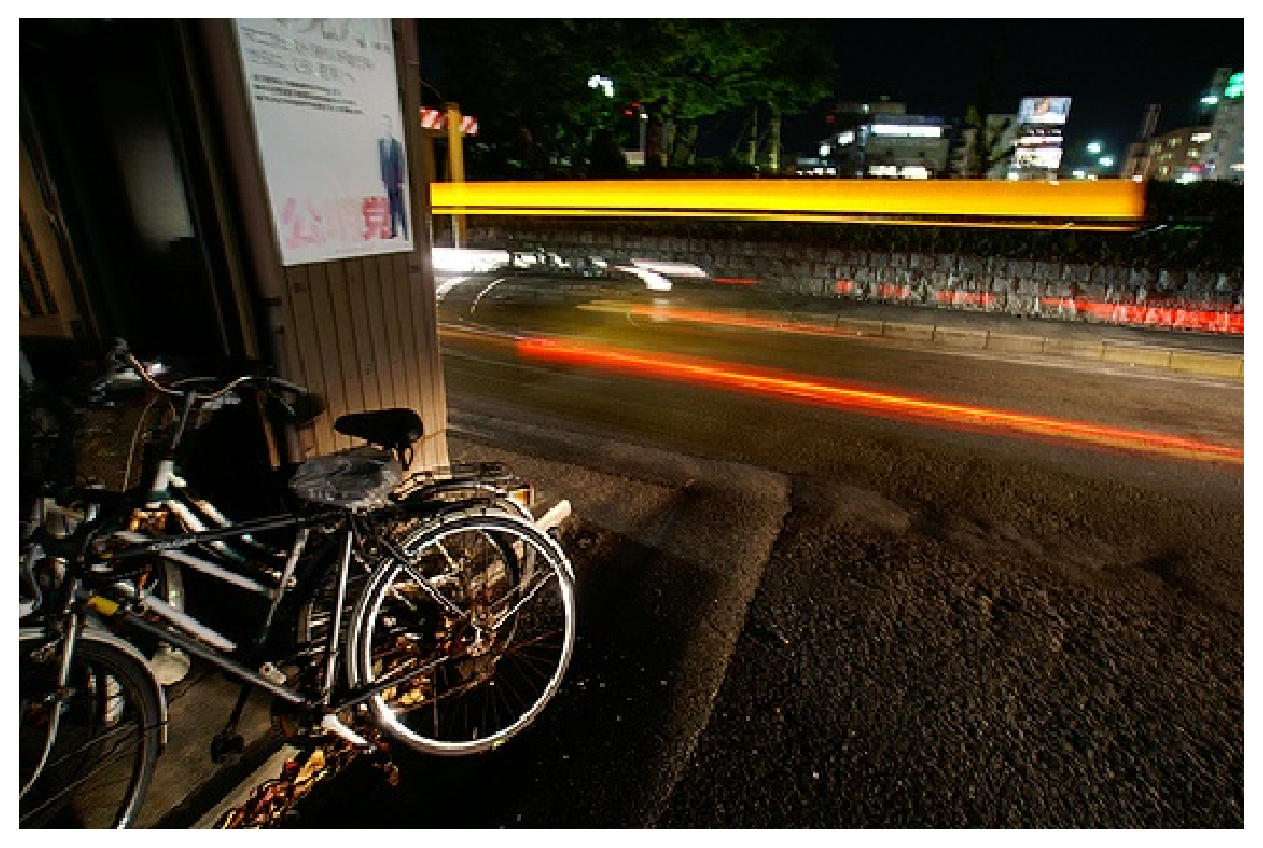
\includegraphics[width=57pt, height=45pt]{./Figures/bike_org.eps}
    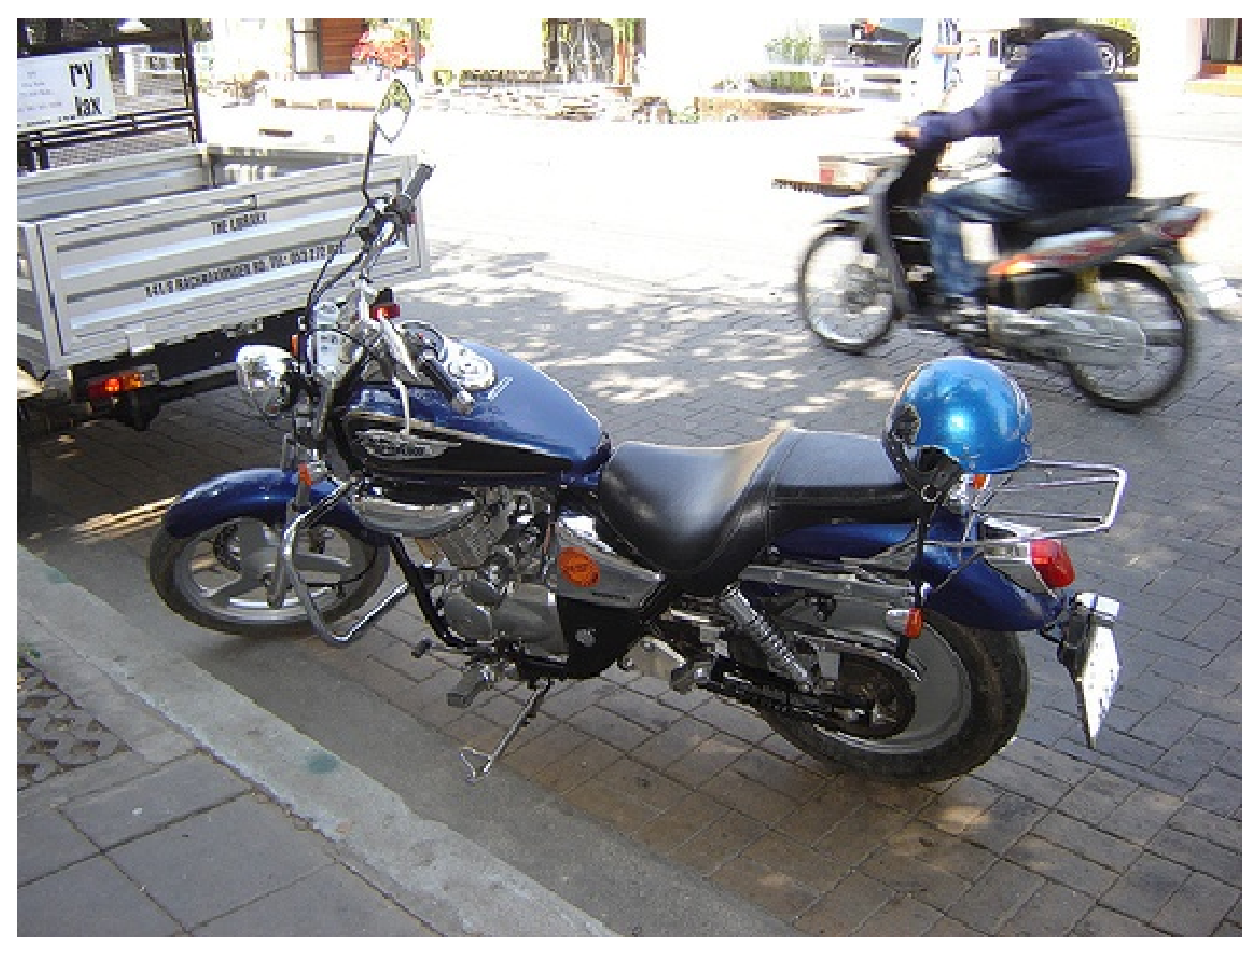
\includegraphics[width=57pt, height=45pt]{./Figures/moto_org.eps}
    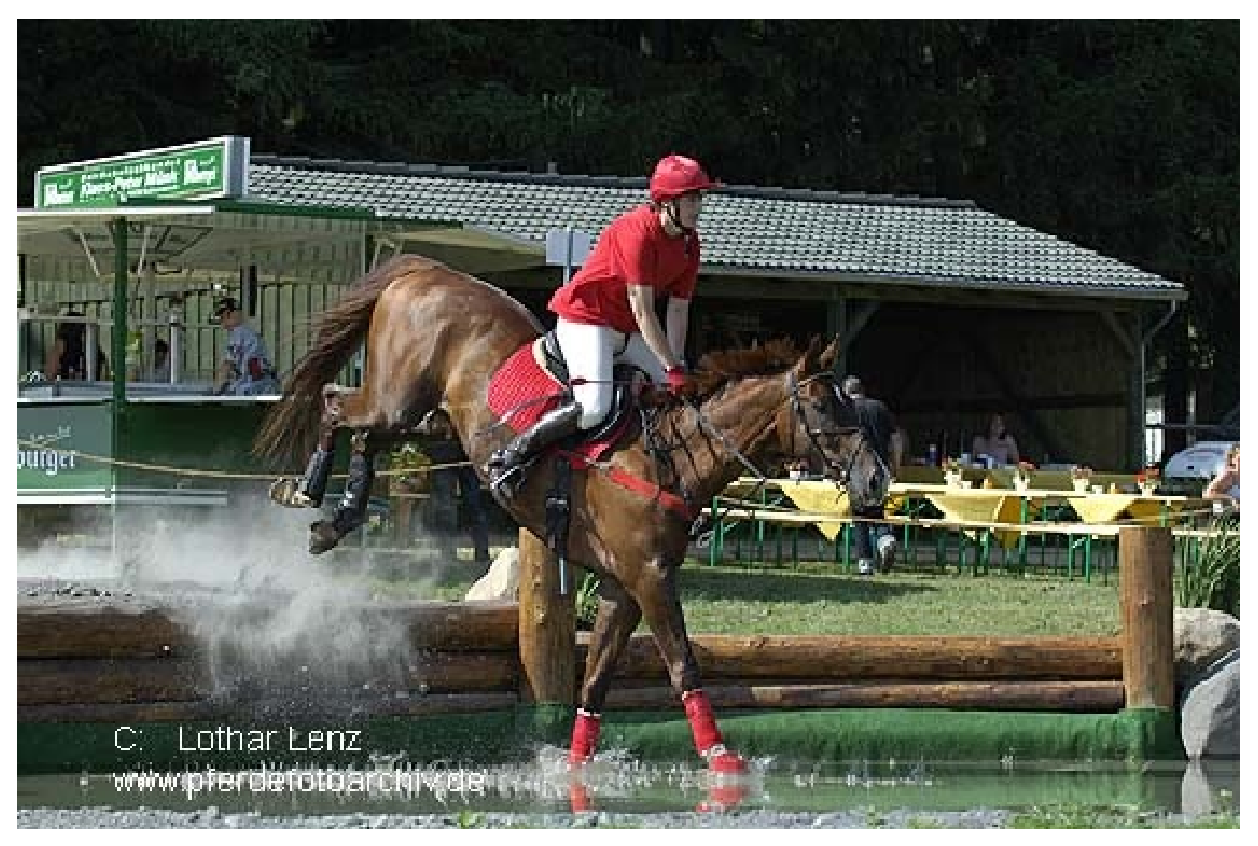
\includegraphics[width=57pt, height=45pt]{./Figures/horse_org.eps}
    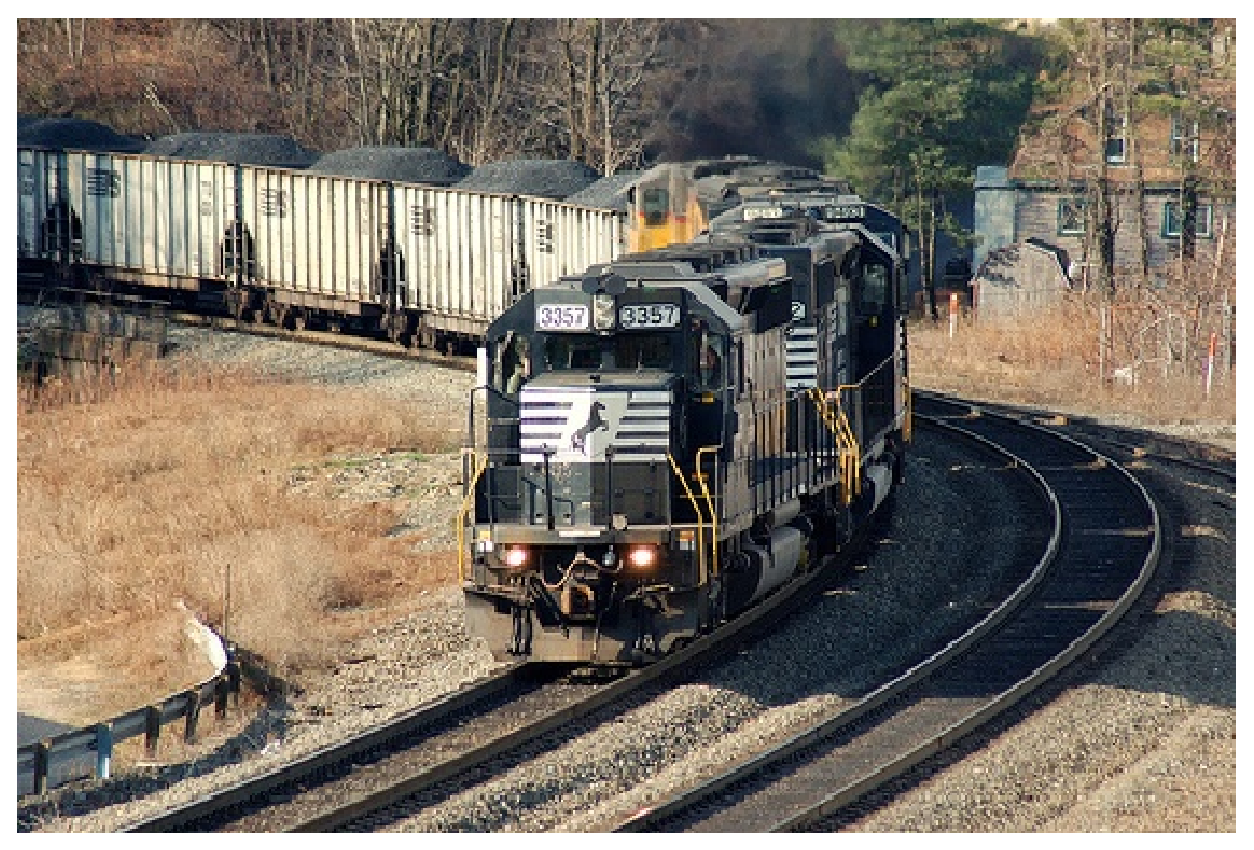
\includegraphics[width=57pt, height=45pt]{./Figures/train_org.eps}
    \label{fig:qualitativegt}
}
\subfigure[Confidence of corresponding class] {
    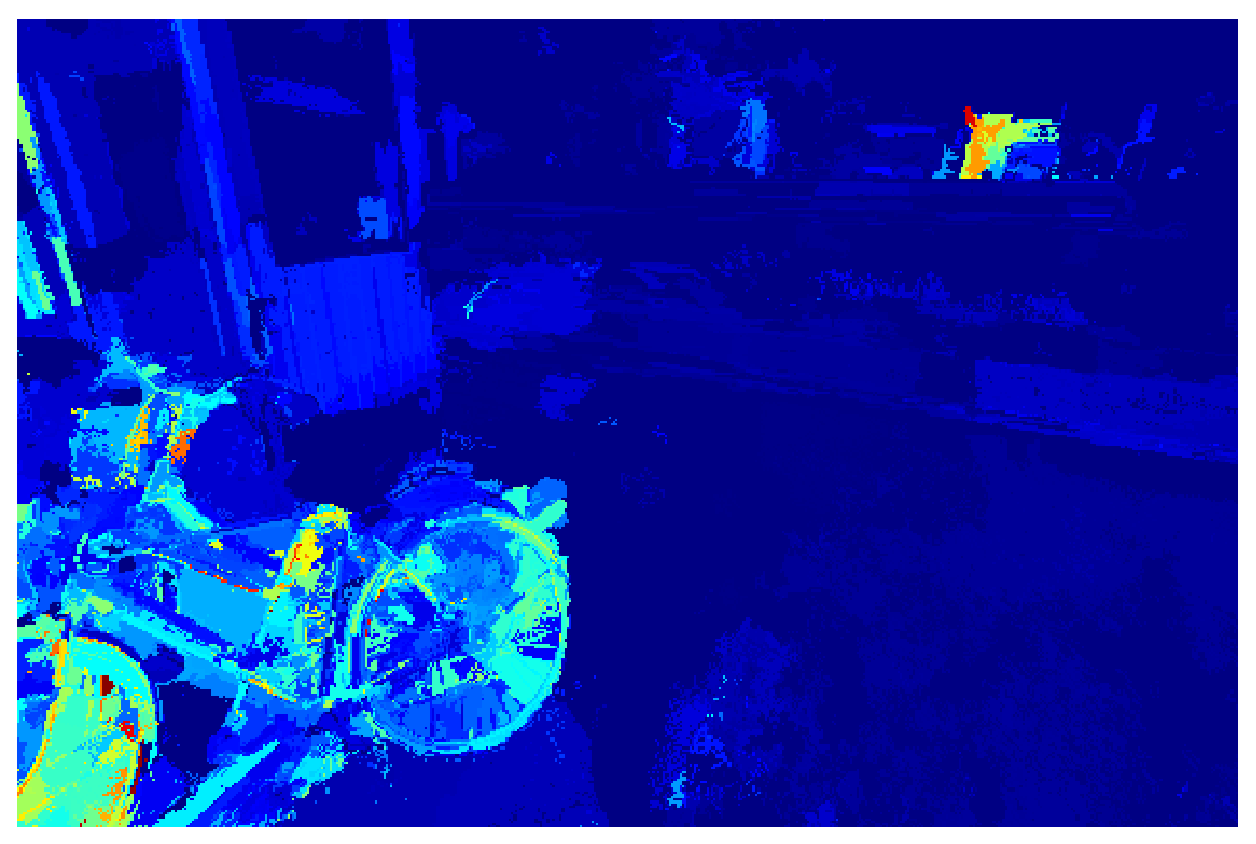
\includegraphics[width=57pt, height=45pt]{./Figures/bike_conf.eps}
    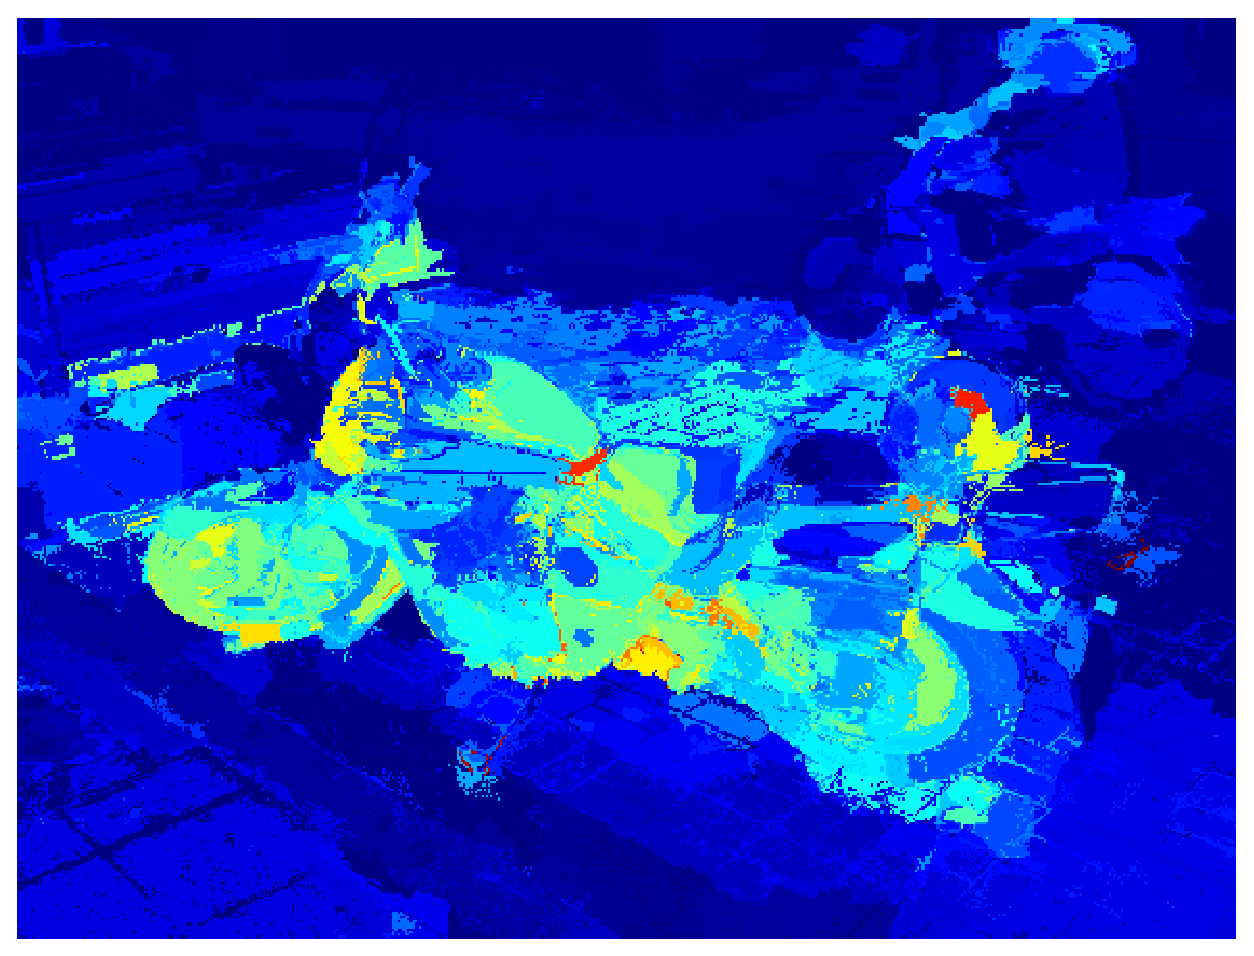
\includegraphics[width=57pt, height=45pt]{./Figures/moto_conf.eps}
    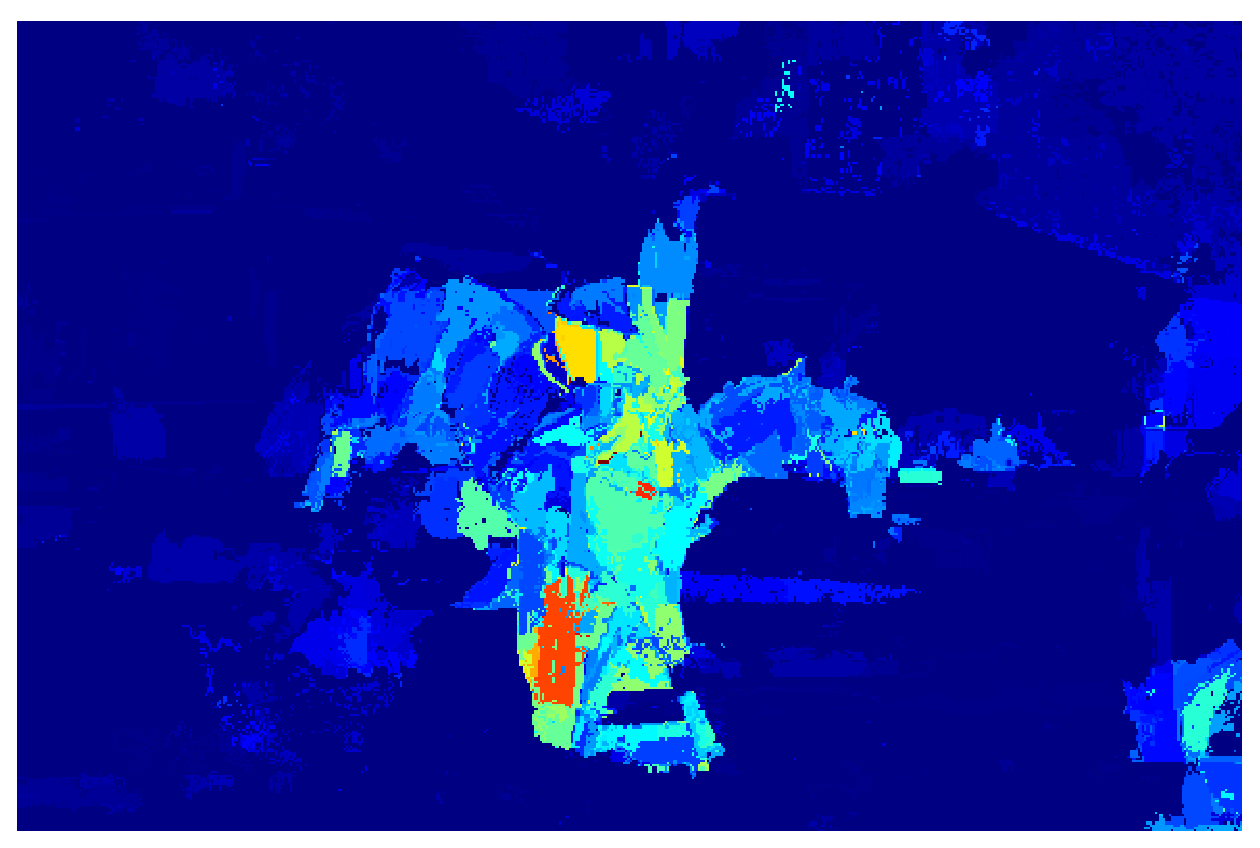
\includegraphics[width=57pt, height=45pt]{./Figures/horse_conf.eps}
    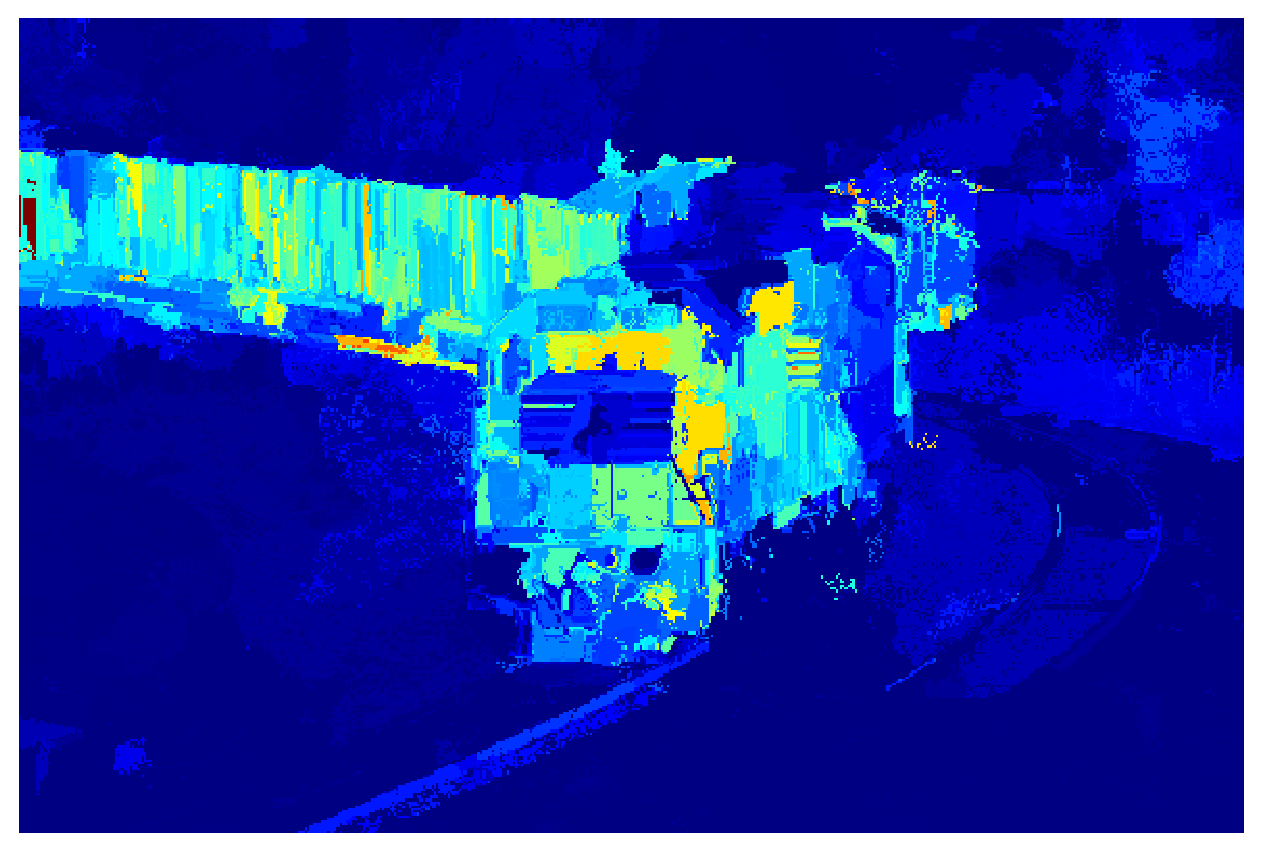
\includegraphics[width=57pt, height=45pt]{./Figures/train_conf.eps}
    \label{fig:qualitativeconf}
}
\centering
\caption{Qualitative results. The higher the intensity of the color the more confident is the classifier about its classification. Best viewed in colors.}
\label{fig:qualitative}
\end{figure}

\section{Conclusions and Future Work}\label{sectionConclusions}

We have demonstrated the effect of using multiple segmentations on improving
the segments and hence improving the applications that use image
segmentations as a prerequisite. We presented a novel framework for recognizing
and segmenting objects. Our approach relies on multiple bottom-up image
segmentations to build another intuitive more accurate image segmentation.
These bottom-up segmentations then support top-down object recognition
and localization. We have shown how these techniques improve the average accuracy
of a challenging dataset. The PASCAL VOC 2007 object segmentation challenge.

We also showed that superpixels are usually not the best level of representation
for objects. They provide very basic information about each segment that don't
usually vary between different object classes. Hence, we showed the effect of
using larger segments on the final object segmentation which was in all cases
better than using superpixels.

We also believe there are still some of the possible extensions that can be added
to our method to help in boosting the results even higher. We show these extensions
with a simple analysis on how they can be done and how it'll affect the results.

One possible extension will be learning weights that are assigned to each segmentation method per category per position.
Currently, our weighting function just assigns fixed constant weights to each position. This can be improved by
learning those weights and assigning the optimal weights for each segmentation method.

Another possible extension is to incorporate image level priors. For example, if the classification
results show that a certain class exist in the image with a certain probability, we can boost the
weights assigned to this class specifically in our voting scheme. Also we can demote other categories
where their concurrent existence with our existing class is unlikely.

One other possible extension is the use of object detection to guide segmentation. In this case our
framework will promote our existing class within the detection bounding box. In other words, within
the bounding box we can recognize only two categories, the detected object and its background.

Finally, we can find other ways for segments ``goodness'' evaluation. For instance, for the JSEG segmentation
\cite{jseg:462311}, the criterion chosen for good segmentations evaluation is the spatial relation existing
between the pixels in the image space. Another way is to use the color boosting algorithm introduced in
\cite{Weijer05boostingcolor} and consider a segment ``good'' if the number of salientpoints is below a certain threshold.

%%%%%%%%%%%%%
%% References
%%%%%%%%%%%%%
{\small
\bibliographystyle{ieee}
\bibliography{egbib}
}
\end{document}
